\documentclass{bioinfo}
\copyrightyear{2015} \pubyear{2015}

\access{Advance Access Publication Date: Day Month Year}
\appnotes{Manuscript Category}
\usepackage{graphicx}

\begin{document}
\firstpage{1}

\subtitle{Subject Section}

\title[MsQuality: Calculation of standardized quality metrics of mass spectrometry data]{MsQuality – an interoperable open-source package for the calculation of standardized quality metrics of mass spectrometry data}

\author[1,$\ast$]{Thomas Naake}
\author[2]{Johannes Rainer}
\author[1]{Wolfgang Huber}


\author[Naake \textit{et~al}.]{Thomas Naake\,$^{\text{\sfb 1}}$, Johannes Rainer,$^{\text{\sfb 2}}$ and Wolfgang Huber\,$^{\text{\sfb 1}*}$}

\address{}

\address{
$^{\text{\sf 1}}$ Genome Biology Unit, European Molecular Biology Laboratory, Heidelberg, 69117, Germany \\
$^{\text{\sf 2}}$ Institute for Biomedicine (Affiliated to the University of L\"ubeck), Eurac Research, Viale Druso 1, 39100 Bolzano, Italy}


\corresp{$^\ast$corresponding author.}

\history{Received on XXXXX; revised on XXXXX; accepted on XXXXX}
\editor{Associate Editor: XXXXXXX}

\abstract{
\textbf{Motivation:} Obtaining high-quality data from mass spectrometry (MS) 
experiments can be challenging due to various factors that can impact the 
accuracy and reproducibility of the data. Quality control (QC) 
techniques are needed to guarantee that the data sets are 
of high quality.\\
\textbf{Results:} The \texttt{MsQuality} R-package calculates and assesses 
various quality metrics for mass spectrometry-derived spectral data at the 
per-sample level. It calculates around 40 low-level quality metrics based on 
the controlled vocabulary of the mzQC quality metrics defined by HUPO-PSI. 
The package helps to identify low-quality samples and track data quality, 
ultimately improving the quality and reproducibility of mass spectrometry 
data for robust scientific discoveries. \\
\textbf{Availability:} MsQuality is implemented in R and is available through 
Bioconductor at https://bioconductor.org/packages/MsQuality.\\
\textbf{Contact:} \href{wolfgang.huber@embl.org}{wolfgang.huber@embl.org}\\
\textbf{Supplementary information:} Supplementary data are available at \textit{Bioinformatics}
online.}

%\keywords{quality control, mass spectrometry, metabolomics, proteomics, R}

\maketitle

Mass spectrometry (MS) is a versatile analytical technique that has been 
adopted in a variety of disciplines, including proteomics, metabolomics, and 
lipidomics. MS enables the identification and quantification of a wide range 
of molecules. Obtaining high-quality data from mass spectrometry experiments 
can be a challenging task, as numerous factors can impact the accuracy and 
reproducibility of the obtained data. To ensure that MS data is of the 
highest quality, it is imperative to implement appropriate quality control 
(QC) techniques to guarantee that the data sets are reliable 
\citep{Koecher2011}.

Here, we introduce the \texttt{MsQuality} R-package, which provides 
functionality to calculate, assess, and track quality metrics for mass 
spectrometry-derived spectral data at the per-sample level. 
The package allows to compute about 40 of the mzQC quality metrics defined by
the Human Proteome Organization-Proteomics Standards Initiative (HUPO-PSI,
hupo-psi.github.io/mzQC). These are calculated on low-level MS data
such as retention times and m/z and associated intensity values.

The package enables tracking and quantification of data quality using 
multiple metrics even on a large scale and helps to identify samples that 
are of low quality, such as those with a high number of missing values, 
ahead-of-time termination of chromatographic runs, or low instrument sensitivity. 
Following the definitions from \cite{Bittremieux2017}, \texttt{MsQuality}
focuses on the calculation of inter-experiment metrics, which can typically be 
obtained by summation from an intra-experiment metric. Examples for
intra-experiment metrics are the chromatogram of the total ion current (TIC) 
over the retention time. Inter-experiment metrics, on the other hand, 
facilitate the comparison of multiple MS runs or experiments, 
e.g. via longitudinal analysis of quality metrics, such as the
fractions of the total retention time required to accumulate a given
percentile of the TIC.

\section{Usage scenario and implementation} \label{usagescenario}

\texttt{MsQuality} offers easy-to-use means of evaluating data quality on a 
per-sample basis, including the identification of low-quality samples 
(e.g. poor intensities, low signal-to-noise ratio), biases and outliers, 
variations in calibration, and batch and confounding effects within datasets
(Fig. \ref{fig:fig1} a and b). 
Utilizing community standards for data representation in mass spectrometry 
defined by HUPO-PSI, \texttt{MsQuality}'s metric calculations enable 
data quality comparison, storage, and facile exchange.

\begin{figure}[ht!]
    \centering
 	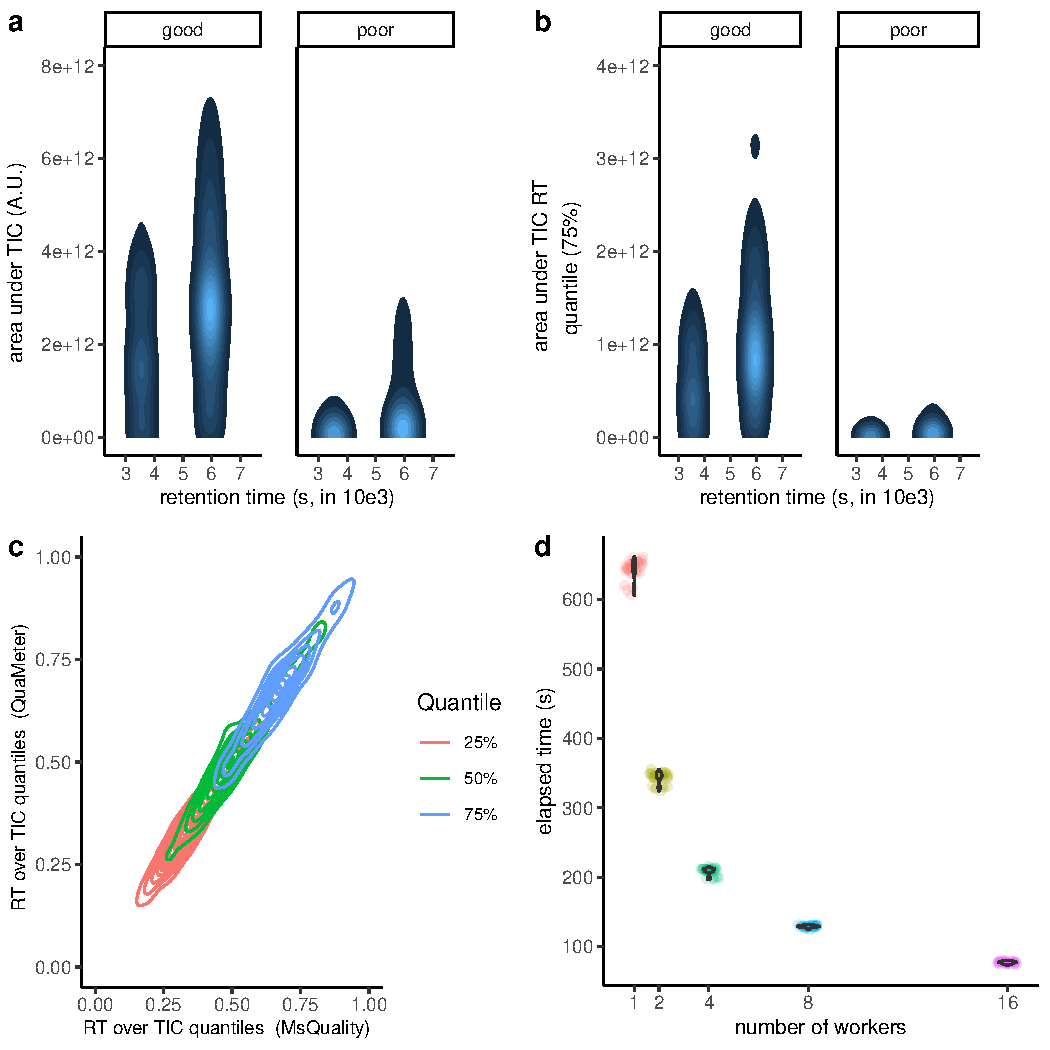
\includegraphics[scale=0.421]{/g/huber/users/naake/GitHub/MsQuality_manuscript/main/figure-main}
 	  \caption{Examples of \texttt{MsQuality} functionality. Metrics are based
 	        on MS1 spectra and one data point is obtained per MS1 spectra.
 	        (a) Area under TIC: The area under the total ion chromatogram. 
            (b) Area under TIC RT quantiles: The area under the total ion
                chromatogram of the retention time quantiles. 
            (c) Comparison of quality metrics calculated by \texttt{MsQuality} 
                and QuaMeter: RT over TIC quantiles. 
            For (a), (b), and (c), the data points are displayed 
                as 2D densities and stratified for high-quality and low-quality
                samples as classified in \cite{Amidan2014} or by the
                quantiles 25\%, 50\%, and 75\%. Brighter areas correspond to 
                high 2D density areas.
            (d) Execution time for the calculation of quality metrics of the 
                data set of \cite{Amidan2014} under parallelization 
                (1, 2, 4, 8, and 16 workers). A.U. arbitrary units.
    } \label{fig:fig1}
\end{figure}

The versatility of \texttt{MsQuality} in calculating metrics extends to a 
wide range of applications, including small-scale studies and long-term 
acquisition of mass spectrometry data. 
The utility of \texttt{MsQuality} is demonstrated through two case studies, 
utilizing a previously published 180 cancer cell line dataset obtained by 
flow injection analysis \citep{Cherkaoui2022} and a liquid 
chromatography(LC)-MS dataset of
the same QC sample \citep{Amidan2014} for long-term quality control.
The tool provides consistent results 
when compared to other data quality tools, such as QuaMeter \citep{Ma2012} 
(Fig. \ref{fig:fig1} c) or MatrixQCvis \citep{Naake2022}. Correlating the 
\texttt{MsQuality} metrics to pre-calculated QuaMeter metrics 
\citep{Amidan2014} showed that 75\% of the analyzed metrics showed Pearson
correlation coefficients over 0.81 and Spearman correlation coefficients over 
0.87 (see the Supplementary Data for further details).

\texttt{MsQuality} is implemented as an open-source R package, relying on the
established \texttt{Spectra} and \texttt{MsExperiment} packages
\citep{Rainer2022} to provide and represent the MS data. By building on these
packages \texttt{MsQuality} thus supports a large variety of data input formats
as well as analyses of very large experiments through the use of data
representations with low memory footprint. Native parallelization enables a fast
and scalable calculation of quality metrics (Fig. \ref{fig:fig1} d, 
see the Supplementary Data for further details).

Finally, \texttt{MsQuality} requires little programmatic interaction
by using only one function call after the instantiation of \texttt{Spectra} or 
\texttt{MsExperiment} objects, thus, is user-friendly 
to calculate the quality metrics.


\section{Conclusion}

The software tool, \texttt{MsQuality}, contributes to the expanding list of 
tools that utilize the \texttt{Spectra/MsExperiment} framework to address 
various stages in the analysis pipeline of mass spectrometry data.
The implementation of \texttt{MsQuality}'s metric calculation is designed
to be user-friendly and streamlined and requires little programmatic 
interaction, facilitating reproducible calculations and evaluations of data 
quality metrics.

By building upon an extensive ecosystem for mass spectrometry data, centered
around the \texttt{Spectra} and \texttt{MsExperiment} packages \citep{Rainer2022},  
\texttt{MsQuality} enables researchers to create seamless analysis workflows 
for rapid, efficient, and standardized evaluation of MS data quality, 
ultimately leading to more robust scientific discoveries in mass spectrometry
workflows.


\section{Acknowledgements}

We acknowledge feedback from the SMART-CARE consortium on usability of 
\texttt{MsQuality} and all developers and maintainers of the R/Bioconductor 
packages \texttt{MsQuality} is built upon. We would like to thank Nicola Zamboni
for his valuable assistance in understanding the files and pointing to the 
required files of the study by Cherkaoui et al. (2022).

\subsection{Author contributions statement}

T.N. conceptualized the R package. T.N. and J.R. implemented the algorithms as 
an R package. T.N. analysed the results. T.N., J.R., and W.H. wrote and 
reviewed the manuscript.

\subsection{Funding}

This work was supported by the Bundesministerium für Bildung und Forschung 
[grant agreement no. 161L0212E].

Conflict of Interest: none declared.




\begin{thebibliography}{}

\bibitem[Amidan \textit{et~al}., 2014]{Amidan2014}
Amidan, B.G. \textit{et~al} (2014) Signatures for mass spectrometry data
quality.
\textit{Proteome Research}, \textbf{13}, 2215--2222.

% \bibitem[Bereman, 2015]{Bereman2015}
% Bereman, M.S. (2015) Tools for Monitoring System Suitability in LC MS/MS 
% Centric Proteomic Experiments.
% \textit{Proteomics}, \textbf{15}, 891--902.

\bibitem[Bittremieux \textit{et~al}., 2017]{Bittremieux2017}
Bittremieux, W. \textit{et~al} (2017) Computational quality control tools for
mass spectrometry proteomics.
\textit{Proteomics}, \textbf{17}, 1--11.

\bibitem[Cherkaoui \textit{et~al}., 2022]{Cherkaoui2022}
Cherkaoui, S. \textit{et~al} (2022) A functional analysis of 180 cancer cell
lines reveals conserved intrinsic metabolic programs.
\textit{Molecular Systems Biology}, \textbf{18}, e11033.

\bibitem[K\"ocher \textit{et~al}., 2011]{Koecher2011}
K\"ocher, T. \textit{et~al} (2011) Quality control in LC-MS/MS.
\textit{Proteomics and Systems Biology}, \textbf{11}, 1026--1030.

% \bibitem[Paulovich \textit{et~al}., 2010]{Paulovich2010}
% Paulovich, A.G. \textit{et~al} (2010) Interlaboratory Study Characterizing a 
% Yeast Performance Standard for Benchmarking LC-MS Platform Performance.
% \textit{Molecular \& Cellular Proteomics}, \textbf{9}, 242--254.

\bibitem[Ma \textit{et~al}., 2012]{Ma2012}
Ma, Z.-Q. \textit{et~al} (2012) QuaMeter: Multivendor Performance Metrics
for LC–MS/MS Proteomics Instrumentation.
\textit{Analytical Chemistry}, \textbf{84}, 5845--5850.

\bibitem[Naake \textit{et~al}., 2022]{Naake2022}
Naake, T. \textit{et~al} (2022) MatrixQCvis: shiny-based interactive data
quality exploration for omics data.
\textit{Bioinformatics}, \textbf{38}, 1181--1182.

\bibitem[Rainer \textit{et~al}., 2022]{Rainer2022}
Rainer, J. \textit{et~al} (2022) A Modular and Expandable Ecosystem for Metabolomics Data Annotation in R.
\textit{Metabolites}, \textbf{12}, 173.

\end{thebibliography}


%\bibliographystyle{natbib}
%\bibliographystyle{achemnat}
%\bibliographystyle{plainnat}
%\bibliographystyle{abbrv}
%\bibliographystyle{bioinformatics}

%\bibliographystyle{plain}

\bibliography{../supplement/document.bib}

\end{document}
 
